\documentclass[12pt]{article}

\usepackage{geometry}
\usepackage{lmodern}
\usepackage{float}
\usepackage{fancyhdr}
\usepackage{amssymb}
\usepackage{hyperref}
\usepackage{natbib}
\usepackage{xcolor}
\usepackage{parskip}
\usepackage{lastpage}
\usepackage{graphicx}
\usepackage{mhchem}
\usepackage{physics}
\usepackage{multirow}
\geometry{a4paper,left=1.5cm,right=1.5cm,top=2.5cm,bottom=2.5cm}

\fancyhf{}
\fancyhead[l]{Team \#15803}
\fancyhead[r]{Page \thepage\ of \pageref{LastPage}}
\pagestyle{fancy}
\setlength{\headheight}{15pt}

\newcommand{\identifierRedFont}[1]{{\huge \textbf{\textcolor{red}{#1}}}}
\newcommand{\todo}[1]{\textbf{[\textcolor{red}{TODO} #1]}}

\parskip=6pt

\begin{document}

\thispagestyle{empty}

\begin{center}
	Team Control Number
	
	\identifierRedFont{15803}

	Problem Chosen
	
	\identifierRedFont{B}

	\textbf{\large 2024} \\
	\textbf{HiMCM}

	\textbf{\small Summary Sheet}
\end{center}

\noindent\rule{\textwidth}{1pt}

\begin{center}
	\section*{Summary}
\end{center}

\newpage

{\center\tableofcontents}

\newpage

\section{Introduction}

\subsection{Background information}

Under the current global trend of technology advancement, high-powered computing (HPC) is gaining rising attention for the increasing demand of computationally intensive tasks such as data science, artificial intelligence (AI) training, and cryptocurrency mining.

It is very common to use a massive number of dedicated hardware with strong computating power for these tasks. Data centers are the specific spaces to hold these hardware. The operation of data centers is usually extremely energy-consuming, with a tremendous demand of electricity to keep the computer systems running and to cool them down.\todo{statistics about electricity} Cryptocurrency mining machine clusters also work similarly to data centers, with all resources dedicated for mining. The intensive use of electricity, contributing heavily to global warming, as well as a lot of other problems, e.g. water usage, e-waste, etc., poses the environmental concerns of HPC.

As sustainability arises as one of the most important development goals in the twenty-first century, it is high time we take action to assess the environmental consequences of HPC and to minimize its negative effects. We proposed an approach to evaluate the environmental impacts due to HPC through mathematical models.

\todo{add more about past researches on energy demands; cites needed}

\todo{dataset and used tools}

\subsection{Restatement of the problems}

\todo{adjust this section later}

\todo{}

\subsection{Our Work}

\todo{}

\section{HPC energy consumption model}

In this section, we model the annual worldwide energy consumption of \textit{high-powered computing} (HPC). HPC includes various computationally intensive tasks, which are mostly carried out by computer systems in data centers and cryptocurrency mining machines. Therefore, it is feasible to estimate the total energy consumption of HPC from these two sectors.

\subsection{Assumptions}
\label{sec_energy_model_assumptions}

\begin{enumerate}
	\item The total power data offered by data center providers reflects the maximum power. \\
	\textbf{Justification:} The data of total power in a data center is typically defined by the machines' design specifications. Therefore, we interpret this as the hard limit of the possible power allocated on the machines.
	
	\item Possible non-HPC data centers are also included. \\
	\textbf{Justification:} Since most data centers are hybrid, it is hard to exactly distinguish between HPC and non-HPC ones. Non-HPC hardware such as storage may also contribute to the process of HPC. Moreover, they share most of the infrastructure with HPC consuming a more significant amount of energy. Therefore, including some possible non-HPC facilities is not likely to create a large impact on the results.
	
	\item All data are from a same, \textit{short-run} scenario where there are no differences in conditions. \\
	\textbf{Justification:} Most of the data we found are statistics or information within or throughout the year 2022 to 2024. We tried to use the latest statistics, but this is not always available since the year of 2024 is not over yet by the time we work on this model. The assumption of the \textit{short-run} data means that we regard all data as taken from a same set of conditions with no development or changes between them; delving into the detailed differences would make the model way too complex and beyond the intended scope.

	\item The utilization rates across different data centers are the same. \\
	\textbf{Justification:} The actual utilization rates across different data centers are not varying very much. Since the emphasis of our model is on the estimation of total energy, the detailed utilization rates on each data center are not of significant interest and neglected.

	\item Bitcoin (BTC) mining is considered as the whole cryptocurrency mining industry. \\
	\textbf{Justification:} By the time we work on this model, Bitcoin (BTC) is the cryptocurrency with the largest capitalization and mining energy consumption. Cryptocurrencies other than BTC, namely \textit{altcoins}, consumes way less energy than BTC mining, especially with the second largest Ethereum (ETH) switched to proof of stake (PoS) instead of the traditional proof of work (PoW) mining. \todo{cite}

	\item Cryptocurrency mining machines are always operating at their \textit{full capacity rate}. \\
	\textbf{Justification:} As a highly-competitive industry, miners are profit-driven and tend to maximize their profits. Mining at the machines' full capacity ensures the maximum output which lowers the averaged fixed costs, such as the costs of mining machines and related infrastructures, and thus maximizes the profits.

	\item All other unlisted source of HPC are not considered. \\
	\textbf{Justification:} We believe the two sectors are enough to give a representation of all HPC activities. Unlisted sources, such as altcoin mining and small-scale server clusters, contributes very little on the total energy consumption.
\end{enumerate}

\subsection{Model overview}

\begin{table}[!t]
	\centering
	\caption{Definition of symbols. Units: TWh: terawatt hours; MW: megawatts; TH: terahashes.}
	\label{table_symbols_q1}
	\begin{tabular}{lll}
		\hline
		\textbf{Symbol} & \textbf{Unit} & \textbf{Description} \\
		\hline
		$E$ & TWh & Total annual energy consumption of all HPC activities. \\
		$E_D$ & TWh & Total annual energy consumption of data centers. \\
		$E_M$ & TWh & Total annual energy consumption of cryptocurrency mining. \\
		$T$ & h & The time duration (in this case, $\rm = 1yr = 8760h$). \\
		$P_i$ & MW & Total maximum power of data center $i$. \\
		$\overline{\rho}$ & -- & Average utilization rate of data centers. \\
		$H$ & TH/s & Total hash rate performed by the network. \\
		$\kappa$ & -- & Multiplier between the average and the optimal mining efficiency. \\
		$\varepsilon_{\rm opt}$ & J/TH & Efficiency of the best mining machine (power per hash rate). \\
		$\overline{\varepsilon}$ & J/TH & Average efficiency among mining machines ($\overline{\varepsilon} = \kappa \varepsilon_{\rm opt}$). \\
		\hline
	\end{tabular}
\end{table}

We define a set of symbols as in Table \ref{table_symbols_q1}. The total annual power consumption of HPC is
\begin{equation}
	E = E_D + E_M,
\end{equation}
which is the sum of energy consumed by data centers and cryptocurrency mining. In this model, some proportional relationships will be intentionally introduced to facilitate the subsequent models.

\subsubsection{Energy consumption of data centers}

The annual energy consumption of data centers \textit{at full capacity} is straightforwardly defined as
\begin{equation}
	E_{D \rm max} = T \sum_i P_i,
\end{equation}
which is the product of the time of a year and the sum of maximum powers of all data centers. To get the case at \textit{average utilization rate}, we simply multiply it by the average utilization rate $\overline{\rho}$:
\begin{equation}
	E_{D \rm avg} = \overline{\rho} E_{D \rm max} = \overline{\rho} T \sum_i P_i.
\end{equation}

\subsubsection{Energy consumption of cryptocurrency mining}

During cryptocurrency mining, many miners join a network to solve blocks. The \textit{hash rate} is a measure of the computational power of a machine, defined as the number of hash calculations performed per unit time. The total hash rate $H$ of a network is the sum of the hash rates of all machines connected to the network, with a higher value representing a higher competition among miners.

A mining machine works at a specific power and holds a specific computational power, or hash rate. The ratio between the working power and its computational power gives its \textit{efficiency} $\varepsilon$, the power required to achieve unit hash rate (in the unit of power per hash rate, or energy per hash).

To calculate the total power $P$ in a network, we multiply the average efficiency $\overline{\varepsilon}$ among all mining machines with the network's total hash rate $H$ \citep{btc_energy}:
\begin{equation}
	P = \overline{\varepsilon} H.
	\label{eq_mining_power}
\end{equation}

Over time, new mining machines with more advanced technologies are produced and slowly take up the market whilst old machines are still being used (economically speaking, they will be used until their outputs are lower than their operating costs). Therefore, the replacement process takes time; the average efficiency is always lower than the efficiency of the latest machine.

We define $\kappa$ as the ratio between the average efficiency $\overline{\varepsilon}$ (among all machines) and the optimal efficiency $\varepsilon_{\rm opt}$ (of the current best model). Equation \ref{eq_mining_power} can be rewritten as
\begin{equation}
	P = \overline{\varepsilon} H = \kappa \varepsilon_{\rm opt} H.
\end{equation}

Finally, we multiply the power with the one-year time $T$ to get the annual energy consumption:
\begin{equation}
	E_M = PT = \kappa \varepsilon_{\rm opt} HT;
	\label{eq_crypto_energy}
\end{equation}
this is both the \textit{full capacity} level and the \textit{average utilization} level since cryptocurrency mining is assumed to be always operating at the maximum utilization possible.

\subsubsection{Total annual energy consumption}

Combining the above equations, the total annual energy consumption at \textit{full capacity} is expressed as
\begin{equation}
	E_{\rm max} = E_{D \rm max} + E_M = T \sum_i P_i + \kappa \varepsilon_{\rm opt} HT,
\end{equation}
and the total annual energy consumption at \textit{average utilization rate} is
\begin{equation}
	E_{\rm avg} = E_{D \rm avg} + E_M = \overline{\rho} T \sum_i P_i + \kappa \varepsilon_{\rm opt} HT.
\end{equation}

\subsection{Assessing the model using current data}

To assess the accuracy of the energy consumption model, we substitute existing data into our model and compare the model's output with the related existing aggregated statistics.

\subsubsection{Data centers}

We acquired data from \textit{datacenters.com}, a website offering detailed information of data centers worldwide. 4342 data centers \citep{datacenters_com} are included, with information of each's name, location, provider, space, total power, etc. Table \ref{table_data_datacenters.com} shows some of the results from the website.

\begin{table}[!t]
	\centering
	\caption{Some records of data center information from \textit{datacenters.com}. Only columns including data related to the model are displayed; names and addresses that are too long are truncated.}
	\label{table_data_datacenters.com}
	\small
	\begin{tabular}{clrrr}
		\hline
		\textbf{ID} & \textbf{Name} & \textbf{Address} & \textbf{Total space} (sqft) & \textbf{Total power} (MW) \\
		\hline
		0 & Equinix: ... & ..., Tokyo, Japan & 58992 & 6.75 \\
		1 & KAO Data: ... & ..., UK & 40000 & 40 \\
		2 & NorthC: Eindhoven ... & ..., Netherlands & 43056 & 4.5 \\
		3 & DC2Scale: ... & ..., France & 15000 & 1.5 \\
		4 & DataBank: ... & ..., TX, USA & 23000 & 0.675 \\
		5 & Digital Realty: ... & ..., Opfikon, Switzerland & 79800 & 5 \\
		6 & Ascenty, ... & ..., São Paulo, Brazil & 22604.21 & 34 \\
		7 & EdgeConnex: ... & ..., Calle Larga, Chile & 116519.33 & 14 \\
		8 & Centersquare: ... & ..., MA, USA & 201590 & 15 \\
		9 & Digital Realty: ... & ..., Tamil Nadu, India & 196000 & 20.4 \\
		$\vdots$ &&&& \\
		4341 & Equinix: ... & ..., São Paulo, Brazil & 52743 & 1.8 \\
		\hline
	\end{tabular}
\end{table}

We plotted the distribution of the data as in Figure \ref{fig_data_datacenters_original}; it is worth mentioning that there are two very significant outlier values (denoted yellow on the top) exceeding $10^6$ megawatts. Obviously, it is improbable for those two data centers to consume about 13 times more power than the sum of all other ones (more intuitively, taking up almost 5\% of the total human power consumption); therefore, the data is very possibly incorrectly recorded or in a wrong unit. We thereby removed the two, and now all data are in a reasonable range, as shown in Figure \ref{fig_data_datacenters_clean}.

\begin{figure}[!t]
	\centering
	\begin{minipage}{0.48\textwidth}
		\centering
		\caption{The original dataset.}
		\label{fig_data_datacenters_original}
		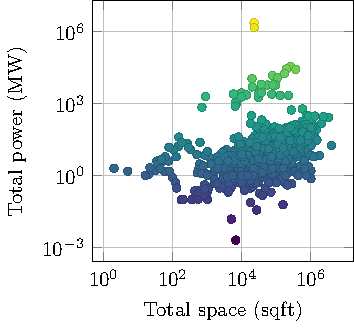
\includegraphics{figures/data/datacenters.pdf}
	\end{minipage}
	\hfill
	\begin{minipage}{0.48\textwidth}
		\centering
		\caption{The dataset with outliers removed.}
		\label{fig_data_datacenters_clean}
		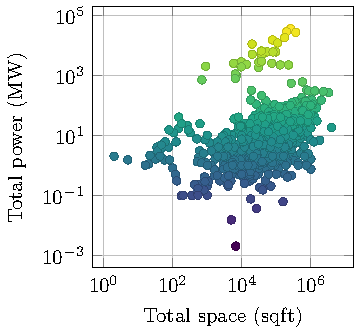
\includegraphics{figures/data/datacenters_clean.pdf}
	\end{minipage}
\end{figure}

We then calculated the sum of the total powers of all data centers without the outliers, yielding $\sum_i P_i = 309,160 \rm MW$. Therefore, the annual energy consumption of data centers at \textit{full capacity} is
\begin{equation}
	E_{D \rm max} = T \sum_i P_i =
	\rm 8,760h \times 309,160MW \approx \mathbf{2,708TWh}.
\end{equation}

The 2024 Kubernetes Cost Benchmark Report \citep{kubernetes_report} reveals that the average utilization rate for Kubernetes server clusters is 13\%. Since Kubernetes is widely used in data centers, this figure is highly representative for general data center utilization. Therefore, we get the annual energy consumption of data centers at \textit{average utilization rate}:
\begin{equation}
	E_{D \rm avg} = \overline{\rho} E_{D \rm max}
	= \rm 13\% \times 2,708TWh \approx \mathbf{352TWh}.
\end{equation}

This falls in the range of world data centers stats \todo{add stats here}.

\subsubsection{Cryptocurrency mining}

Using the recent (November 2024) Bitcoin network data \citep{hashrate}, the total hash rate $H \approx \rm 750,000,000TH/s$. The currently most advanced mining machine is Antminer S21 \citep{best_miner}, with required power of 3531W and a hash rate of 300TH/s, giving the efficiency
\begin{equation}
	\varepsilon_{\rm opt} = \rm \frac{3531W}{300TH/s} = 11.77J/TH.
\end{equation}

According to an examination of a real-world mine \citep{miner_avg_eff}, the actual power consumption of the mine is about 70\% higher than the theoretical optimum, thus the multiplier $\kappa = 1.7$. This gives the total annual energy consumption of cryptocurrency mining:
\begin{equation}
	E_M = \kappa \varepsilon_{\rm opt} HT
	= \rm 1.7 \times 11.77J/TH \times 750,000,000TH/s \times 8,760h \approx \mathbf{131TWh},
\end{equation}
which also falls in the range \todo{range}.

\subsubsection{Evaluation}

\todo{whether necessary?}

\section{HPC carbon emission model}

In this section, we model the carbon emissions of all HPC activities based on the previous energy consumption model. \todo{write more}

We additionally defined several symbols in this model, as shown in Table \ref{table_symbols_q2}.

\subsection{Assumptions}

Assumptions in Section \ref{sec_energy_model_assumptions} are still used in this section. Here are the additional assumptions:

\begin{enumerate}
	\item The energy mix of a data center is exactly the same as the energy mix of the country it is in. \\
	\textbf{Justification:} Most data centers are directly connected to the national electrical grid, which's electricity comes from a mixed source. The detailed investigation of the energy mix at each location is far beyond the scope of this model; we hence simplify this to a uniform national averaged distribution of electricity source.

	\item All data, such as total power and energy mix, are discretized for each year, i.e., within one year, the data is uniform and does not change. \\
	\textbf{Justification:} This assumption is to match most of the data that comes in the form of annual statistics. Since the model aims to provide insights on the current state and long-term future predictions of carbon emissions, ignoring the temporal variations within one year simplifies the model and makes it easier to be implemented from data.

	\item Each type of energy source has a same fixed carbon emission per unit energy in every country and does not change over time. \\
	\textbf{Justification:} In reality, a same type of energy source may have different carbon emissions in different places (e.g., the difference in the effectiveness of wind power due to different natural conditions at different sites); technological advancements also reduces carbon emissions (e.g., by increasing the efficiency of resource usages). To accurately model these, we would need time-varying emissions data at province level or even city level; such differences are ignored because they would make the model too complex while not creating any significant change.

	\item The HPC industry is a ever-developing industry throughout the timeframe we are modeling. \\
	\textbf{Justification:} It is impossible to determine whether, why and when the industry will continue to expand, mature and stagnate, or decay in the future. Since past data of HPC shows its consistent growth in the past years and we are investigating its development over a medium time span (compared with the time range of available data), it is reasonable for us to assume the persistence of this trend and simplify the model.
\end{enumerate}

\begin{table}[!t]
	\centering
	\caption{Definition of new symbols. The symbol $x \in \left\{ \rm F, N, R \right\}$ stands for the method of electricity production, respectively fossil fuels (F), nuclear energy (N), and renewable energy (R).}
	\label{table_symbols_q2}
	\begin{tabular}{lll}
		\hline
		\textbf{Symbol} & \textbf{Unit} & \textbf{Description} \\
		\hline
		$\Psi$ & t & Total annual carbon emission of all HPC activities. \\
		$\Psi_D$ & t & Total annual carbon emission of data centers. \\
		$\Psi_M$ & t & Total annual carbon emission of cryptocurrency mining. \\
		$\Xi_{i,\rm T}$ & TWh & Total annual electricity production of country $i$. \\
		$\Xi_{i,x}$ & TWh & Annual electricity production of country $i$ using method $x$. \\
		$M_{x}$ & t/TWh & Mass of \ce{CO2} created per unit of electricity produced using method $x$. \\
		$C_{i}$ & t/TWh & Carbon emission per unit electricity produced in country $i$. \\
		$\zeta_{i,x}$ & -- & Proportion of electricity production of country $i$ using method $x$. \\
		$\zeta_{{\rm M},x}$ & -- & Proportion of electricity for crypto. mining produced using method $x$. \\
		$t$ & -- & A particular year in A.D. \\
		\hline
	\end{tabular}
\end{table}

\subsection{Carbon emissions at a fixed time (present)}

Similarly, we calculate the total emissions through adding up the two sectors. We categorize all energy sources that are used to produce electricity into three types: fossil fuels (F), nuclear energy (N), and renewable energy (R). In this section, all calculations will use the current data.

\subsubsection{Carbon emission of data centers}

Suppose the electricity production of country $i$ (with a total of $n$ countries) from energy type $x$ is $\Xi_{i,x}$, we have the mix and total energy for the production of electricity of all countries:
\begin{equation}
	\vb{\Xi} = \begin{bmatrix}
		\Xi_{1,\rm F} & \Xi_{1,\rm N} & \Xi_{1,\rm R} \\
		\Xi_{2,\rm F} & \Xi_{2,\rm N} & \Xi_{2,\rm R} \\
		\vdots & \vdots & \vdots \\
		\Xi_{n,\rm F} & \Xi_{n,\rm N} & \Xi_{n,\rm R} \\
	\end{bmatrix}; \quad
	\vb{\Xi_T}
	= \begin{bmatrix}
		\Xi_{1,\rm T} \\
		\Xi_{2,\rm T} \\
		\vdots \\
		\Xi_{n,\rm T} \\
	\end{bmatrix}
	= \begin{bmatrix}
		\Xi_{1,\rm F} + \Xi_{1,\rm N} + \Xi_{1,\rm R} \\
		\Xi_{2,\rm F} + \Xi_{2,\rm N} + \Xi_{2,\rm R} \\
		\vdots \\
		\Xi_{n,\rm F} + \Xi_{n,\rm N} + \Xi_{n,\rm R} \\
	\end{bmatrix}
	= \vb{\Xi} \vb{1}.
\end{equation}

Therefore, we define the proportions of the electricity produced from each energy source in all electricity production for each country, $\boldsymbol{\zeta} \in \mathbb{R}^{n \times 3}$, as
\begin{equation}
	\zeta_{i, x}
	= \frac{\Xi_{i, x}}{\Xi_{i,\rm T}}
	= \frac{\Xi_{i, x}}{\Xi_{i,\rm F} + \Xi_{i,\rm N} + \Xi_{i,\rm R}}, \quad
	\left(
		x \in \left\{ \rm F, N, R \right\}
	\right).
\end{equation}

For the mass of \ce{CO2} created per unit of electricity
\begin{equation}
	\vb{M} = \begin{bmatrix}
		M_{\rm F} \\
		M_{\rm N} \\
		M_{\rm R} \\
	\end{bmatrix},
\end{equation}
the energy mix proportions $\boldsymbol{\zeta}$ are the weights on each energy type; through linear combination, we calculate the weighted average carbon emission per unit electricity in each country as
\begin{equation}
	\vb{C} = \boldsymbol{\zeta} \vb{M}.
\end{equation}

Since we already have the detailed information of all data centers, we can calculate the total capacity power of data centers in each country as
\begin{equation}
	\vb{P} = \begin{bmatrix}
		\sum_{P_i \rm\;in\;country\;1} P_i \\
		\sum_{P_i \rm\;in\;country\;2} P_i \\
		\vdots \\
		\sum_{P_i \rm\;in\;country\;n} P_i \\
	\end{bmatrix},
\end{equation}
giving the total \textit{real} energy consumption due to data centers in each country
\begin{equation}
	\vb{E_D} = \overline{\rho} T \vb{P},
\end{equation}
where $\overline{\rho}$ is the average utilization rate and $T$ is the time period (one year).

Through linear combination, we deduce the total annual carbon emissions worldwide due to data centers by calculating the multiplication of annual energy and carbon emission per energy:
\begin{equation}
	\Psi_D = \vb{E_D}^\top \vb{C} = \overline{\rho} T \vb{P}^\top \boldsymbol{\zeta} \vb{M}.
\end{equation}

\subsubsection{Carbon emission of cryptocurrency mining}

The industry of cryptocurrency mining is separated mainly for the difficulty in identifying country-wise energy mix. However, the energy mix of the industry as a whole is feasible. We could model the industry in a way similar to modeling another country.

Previously, we have calculated that the annual energy consumption because of cryptocurrency mining is $E_M = \kappa \varepsilon_{\rm opt} HT$. Similarly, we can calculate the carbon emission per unit of electricity as
\begin{equation}
	\vb{C_M} = \boldsymbol{\rm \zeta_M} \vb{M}, \quad
	\left(
		\boldsymbol{\rm \zeta_M} =
		\begin{bmatrix}
			\zeta_{\rm M, F} & \zeta_{\rm M, N} & \zeta_{\rm M, R} \\
		\end{bmatrix}
	\right),
\end{equation}
and therefore, the total carbon emission due to cryptocurrency mining can be defined:
\begin{equation}
	\Psi_M = E_M \vb{C_M} = \kappa \varepsilon_{\rm opt} HT \boldsymbol{\rm \zeta_M} \vb{M}.
\end{equation}

\subsubsection{Results and evaluation}

We add up the two sectors to find the total annual carbon emission of HPC:
\begin{equation}
	\Psi = \Psi_D + \Psi_M
	= \overline{\rho} T \vb{P}^\top \boldsymbol{\zeta} \vb{M}
		+ \kappa \varepsilon_{\rm opt} HT \boldsymbol{\rm \zeta_M} \vb{M}.
\end{equation}

We use the World Energy Balances 2024 Highlights (free extract) dataset \citep{energy_mix_dataset} offered by the International Energy Agency (IEA). The dataset includes comprehensive energy mix data over the past fifty years (since 1971) in many countries and broader regions, including total electricity production and production from fossil fuels, nuclear energy, and renewable energy, as exampled in Table \ref{table_iea_energy_dataset}. Figure \ref{fig_emission_data_availability} shows the most accurate data available from the dataset for each country. Countries having the most data centers, such as the U.S., western European countries, China, Japan, Singapore, etc., all have their own country-specific data available. Therefore, the dataset is highly reliable for modeling the energy structure used by data centers worldwide.

\begin{figure}[!t]
	\centering
	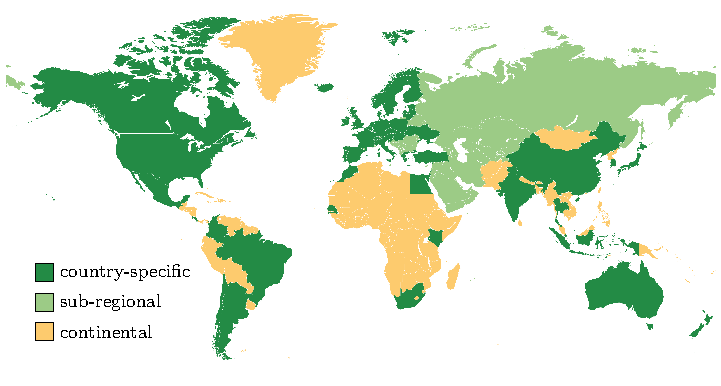
\includegraphics{figures/data/emission_map.pdf}
	\vspace*{-0.5cm}
	\caption{Detailed energy mix data availability in each country.}
	\label{fig_emission_data_availability}
\end{figure}

\begin{table}[!t]
	\centering
	\caption{An extract from the IEA World Energy Balances 2024 Highlights dataset.}
	\label{table_iea_energy_dataset}
	\small
	\begin{tabular}{cllrrrrr}
		\hline
		\multirow{2}*{\textbf{Entry}} & \multirow{2}*{\textbf{Country}} & \multirow{2}*{\textbf{Energy Type}} & \multicolumn{5}{c}{\textbf{Electricity output} (GWh)} \\
		&&& \textbf{1971} & \textbf{1972} & $\cdots$ & \textbf{2022} & $\mathbf{2023}^{\dagger}$ \\
		\hline
		1 & Australia & Fossil fuels & 41201 & 43730 & $\cdots$ & 187536 & 181363 \\
		2 & Australia & Nuclear & 0 & 0 & $\cdots$ & 0 & 0 \\
		3 & Australia & Renewable sources & 11844 & 11853 & $\cdots$ & 83282 & 92216 \\
		4 & Australia & Total & 53045 & 55583 & $\cdots$ & 270818 & 273579 \\
		5 & Austria & Fossil fuels & 11752 & 11939 & $\cdots$ & 13509 & 10205 \\
		6 & Austria & Nuclear & 0 & 0 & $\cdots$ & 0 & 0 \\
		7 & Austria & Renewable sources & 16450 & 16986 & $\cdots$ & 50432 & 59397 \\
		8 & Austria & Total & 28202 & 28925 & $\cdots$ & 64713 & 70301 \\
		$\vdots$ \\
		244 & World & Total & 5256947 & 5698376 & $\cdots$ & 29143442 & -- \\
		\hline
	\end{tabular}
\end{table}

We acquired data for power sector emissions worldwide from Ember \citep{emission_dataset}, including carbon emissions due to coal, gas, other fossil, bioenergy, hydro, solar, wind, nuclear, and other renewables, from the year 2000 to 2023. We extracted the data of 2022: 13,665.56Mt from fossil fuels, 13.61Mt from nuclear energy, and 338.61Mt from renewable energies.

Using data from IEA, we know that in 2022 the world produced 17,772,682GWh, 2,685,464GWh, and 8,559,418GWh, respectively, from the three sources. By dividing the emission with the electricity produced, we get the carbon emission created per unit of electricity in 2022 (in t/TWh):
\begin{equation}
	\vb{M} = \begin{bmatrix}
		768,908 \\ 5,068 \\ 39,560
	\end{bmatrix}.
\end{equation}

Taking all these data, we have
\begin{equation}
	\Psi_D
	= \overline{\rho} T \vb{P}^\top \boldsymbol{\zeta} \vb{M}
	= 13\% \times 1 {\rm yr} \times 1.975 {\rm Mt/h} = 2249 {\rm Mt}
\end{equation}
\ce{CO2} (Mt: million tons) emitted due to data centers.

\begin{figure}[!t]
	\centering
	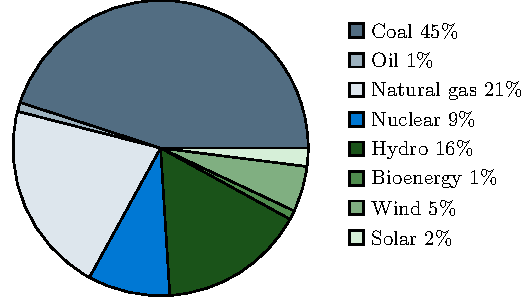
\includegraphics{figures/data/bitcoin_mix.pdf}
	\caption{Energy mix of Bitcoin mining.}
	\label{fig_bitcoin_mix}
\end{figure}

The energy mix used to supply Bitcoin mining is shown in Figure \ref{fig_bitcoin_mix} \citep{bitcoin_mix}. The energy consumption of the industry is 67\% from fossil fuels, 9\% from nuclear energy, and 24\% from renewable sources. Therefore, we calculate the carbon emission of cryptocurrency mining as
\begin{equation}
	\Psi_M = E_M \boldsymbol{\rm \zeta_M} \vb{M}
	= 131 {\rm TWh} \cdot \begin{bmatrix}
		0.67 & 0.09 & 0.24
	\end{bmatrix}\begin{bmatrix}
		768,908 \\ 5,068 \\ 39,560
	\end{bmatrix} {\rm t/TWh}
	= 68.8 {\rm Mt};
\end{equation}
hence, the total carbon emission of HPC at present is
\begin{equation}
	\Psi = \Psi_D + \Psi_M = 2,249 + 68.8 = 2,317.8 {\rm Mt}.
\end{equation}

\subsection{Change in carbon emission over time}

Previously, we calculated the carbon emissions created by HPC at present from several components. By modeling the trends of these components' changes over time, we will construct a model for the future predictions.

\subsubsection{Modeling the change of data centers}

Google is one of the largest firms dominating the market of HPC data centers. We consider it as a reliable representative of the whole industry.

From Google 2024 Environmental Report \citep{google_report}, we have Google's annual energy consumption from 2011 to 2023. The data is plotted in Figure \ref{fig_google} (left). Energy consumption is directly related to the expansion of the industry. From the graph, we can identify an increasing rate of increment in annual energy consumption. This is typically defined by a exponential relationship where there is a constant rate of increasing proportion, i.e., constant ratio between two consecutive years.

\begin{figure}[!t]
	\centering
	\caption{Trend of Google's annual energy consumption from financial year 2011 to 2023. \textbf{Left:} the real data and the exponential fit deduced from the linear fit of the post-log data in the right side. \textbf{Right:} data normalized using natural logarithm and the linear regression on the processed data.}
	\label{fig_google}
	\medskip
	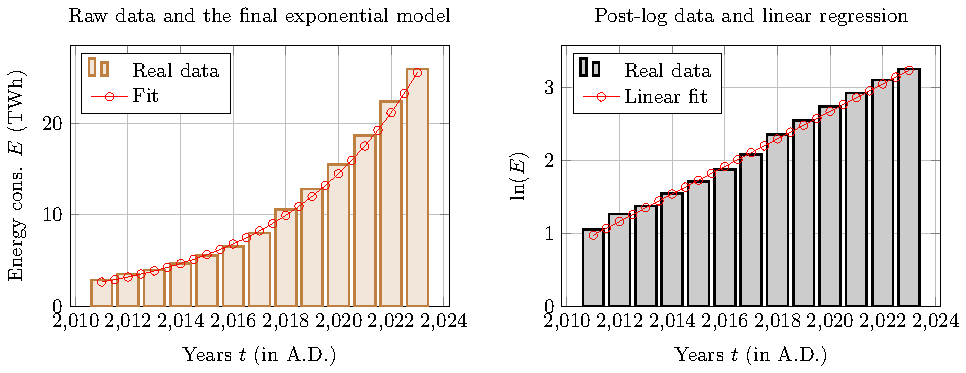
\includegraphics{figures/trends/google.pdf}	
\end{figure}

We thereby calculate the natural logarithm of each data to linearize the trend, as shown in Figure \ref{fig_google} (right). It is obvious that the data is now almost perfectly following a linear trend; therefore, the exponential relationship exists and is a proper way to model the change. Through linear regression (having a correlation of $r \approx 0.99$), we have
\begin{equation}
	\ln \left(E(t)\right) = 0.1887t - 378.5;
\end{equation}
therefore,
\begin{equation}
	E(t) = \exp \left(0.1887t - 378.5\right) = 4.1643 \times 10^{-165} \cdot \exp \left(0.1887t\right).
\end{equation}

Thus, we can calculate the annual increment multiplier $r$ as
\begin{equation}
	r = \frac{E\left(t + 1\right)}{E(t)}
	= \frac{\exp \left(0.1887\left(t + 1\right) - 378.5\right)}{\exp \left(0.1887t - 378.5\right)}
	= \exp \left(0.1887\right).
\end{equation}

Using the previously calculated data of current (2024) global energy consumption of 352TWh from HPC data centers, we can model that
\begin{equation}
	\begin{aligned}
		E_D(t) &= E_D(2024) \cdot r^{t - 2024} = 352 \cdot \exp \left(0.1887(t - 2024)\right) \\
		&= 4.7531 \times 10^{-164} \cdot \exp \left(0.1887t\right),
	\end{aligned}
\end{equation}
for any year $t$. Figure \ref{fig_energy_datacenter} shows the calculated numerical values.

\begin{figure}[!t]
	\centering
	\caption{Estimated energy consumption due to HPC data centers.}
	\label{fig_energy_datacenter}
	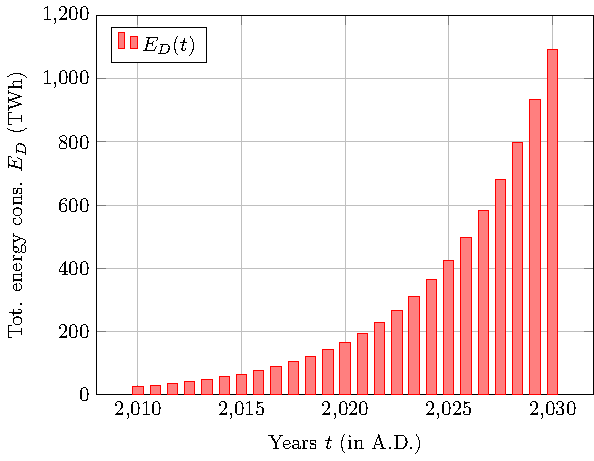
\includegraphics{figures/trends/datacenter_energy.pdf}
\end{figure}

\subsubsection{Modeling the change of cryptocurrency mining}

As deduced in Equation \ref{eq_crypto_energy}, $E_M = \kappa \varepsilon_{\rm opt} HT$. We assume the ratio $\kappa$ to be constant over time. Since our model will be mostly applied to a medium timeframe, $\kappa$, mainly dependent on the distribution of hardware types, are not likely to fluctuate rapidly as the best efficiency of hardware $\varepsilon_{\rm opt}$ or the total hash rate $H$. We thereby model the change in $\varepsilon_{\rm opt}$ and $H$ over time $t$ respectively.

To investigate the trend of the development of the most energy-efficient cryptocurrency mining machine, we aggregated the various lists of data of all mining machines from a range of hardware vendors, researches, and online cryptocurrency-related databases, for the year of 2015 \citep{best_miner_2015}, 2017 \citep{btc_energy}, 2021 \citep{best_miner_2021}, 2022 \citep{best_miner_2022}, 2023 \citep{best_miner_2023}, and 2024 \citep{best_miner}. The extracted data of the miners with the best (smallest) efficiency, which is defined as $\varepsilon = P / H$, is presented in Table \ref{table_best_miners}.

\begin{table}[!t]
	\centering
	\caption{List of the best cryptocurrency mining machine: powers, hash rates, and efficiencies.}
	\label{table_best_miners}
	\small
	\begin{tabular}{c|lrr|r}
		\hline
		\textbf{Year} & \textbf{Model} & $\boldsymbol{P}$ (W) & $\boldsymbol{H}$ (TH/s) & $\boldsymbol{\varepsilon}$ (J/TH)\\
		\hline
		2015 & Antminer S7 & 1,293 & 4.73 & 273.4 \\
		2017 & Antminer S9 & 1,372 & 14 & 98.0 \\
		2021 & Antminer S19 Pro & 3,250 & 110 & 29.5 \\
		2022 & Antminer S19 XP & 3,010 & 140 & 21.5 \\
		2023 & Antminer S19 XP Hyd & 5,304 & 255 & 20.8 \\
		2024 & Antminer S21 & 3,531 & 300 & 11.8 \\
		\hline
	\end{tabular}
\end{table}

\begin{figure}[!t]
	\centering
	\caption{The trend of cryptocurrency miner's best efficiency $\varepsilon_{\rm opt}$ over years. \textbf{Left:} the real data and the exponential fit calculated from the linear fit result of post-log data in the right side. \textbf{Right:} data normalized using natural logarithm with the consequential linear fit on post-log data.}
	\label{fig_miner_trend}
	\medskip
	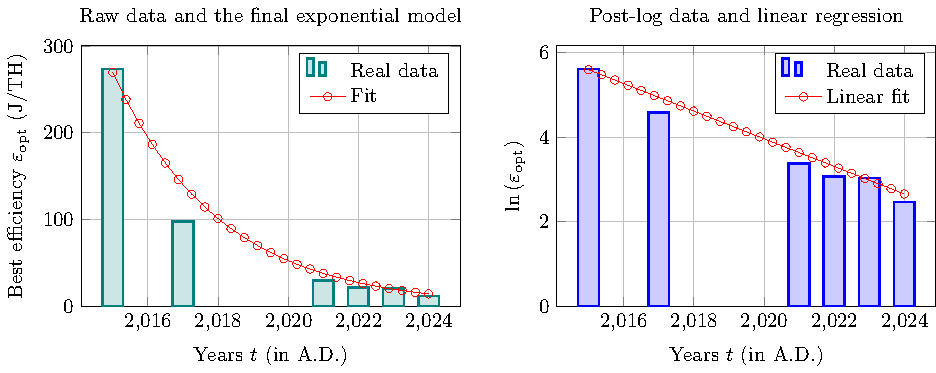
\includegraphics{figures/trends/miner.pdf}
\end{figure}

As illustrated in the Green500 list from the TOP500 list of supercomputers \citep{top500}, the growth of computational performance per power consumed is exponential. The efficiency $\varepsilon$ defined in this research, which is the ratio of power to hash rate, is the reciprocal of the performance per power; this makes $1/\varepsilon_{\rm opt}$ have an exponential growth over time, i.e., $\varepsilon_{\rm opt}$ would decay exponentially over time (since $1/e^x = e^{-x}$).

A straightforward approach to model the exponential relationship would be linearization of the data. We take the natural logarithm values of the efficiencies, $\ln\left(\varepsilon_{\rm opt}\right)$, and find its relationship with the time $t$, as shown in Figure \ref{fig_miner_trend}. Through linear regression, we get
\begin{equation}
	\ln\left(\varepsilon_{\rm opt} (t)\right) = -0.3268t + 664.1,
\end{equation}
with a correlation of $r \approx -0.99$, and hence the efficiency can be modeled as
\begin{align}
	\varepsilon_{\rm opt} (t) = \exp \left(-0.3268t + 664.1\right)
	&= 2.6 \times 10^{288} \cdot \exp \left(-0.3268t\right) {\rm J/TH} \\
	&= 2.6 \times 10^{276} \cdot \exp \left(-0.3268t\right) {\rm TJ/TH}.
	\label{eq_efficiency}
\end{align}

The the Bitcoin network's total hash rate data \citep{hashrate} is plotted in Figure \ref{fig_total_hashrate}, starting from January 2009, the time when Bitcoin was created. The total hash rate increases with faster rates over time. Despite having small fluctuations, the pattern should follow either an exponential model (constantly increasing proportion) or a power function model (growth with limiting resources).

\begin{figure}[!t]
	\centering
	\caption{Total hash rate of the Bitcoin network over time and comparison across models. January 10, 2009 is selected as the day 0. \textbf{Left:} the ground truth. \textbf{Right:} comparison between the exponential model and the power function model, displayed in linear axis (top) and log scaled axis (bottom).}
	\label{fig_total_hashrate}
	\medskip
	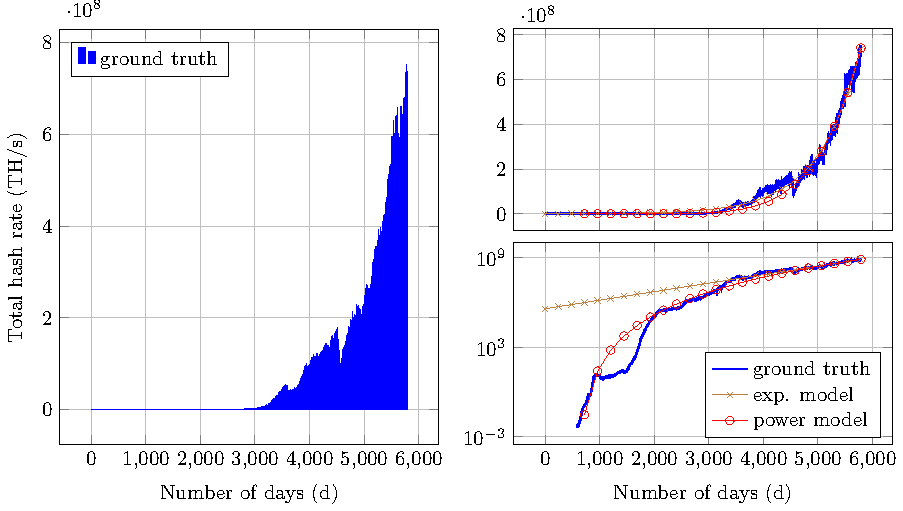
\includegraphics{figures/trends/bitcoin_hashrate.pdf}
\end{figure}

From Figure \ref{fig_total_hashrate} (right), we see that both the exponential model and the power function model showcase a decent capture of the trend (both with a correlation $r \approx 0.99$). However, when the models are compared within a log scaled $y$-axis, the data actually ``bends'' and does not follow a constantly increasing magnitude. The exponential model has deviations with the data trend, whereas the power function almost perfectly matches the data. Therefore, it can be concluded that the total hash rate follows the model
\begin{equation}
	H = 3.087 \times 10^{-16} \cdot (x - 588)^{6.561} \rm TH/s,
\end{equation}
where $x$ is the number of days starting from January 10, 2009. Convert $x$ to years $t$ (A.D.) assuming 365 days every year: $t = 2009 + \frac{1}{365}(x + 10) \Rightarrow x = 365 t - 733295$. Therefore,
\begin{equation}
	H(t) = 19.9867 \left( t - 2,010.6384 \right)^{6.561} \rm TH/s.
	\label{eq_hash_rate}
\end{equation}

Combining Equation \ref{eq_efficiency} and Equation \ref{eq_hash_rate}, we get the model for the total energy consumed by cryptocurrency mining over time:
\begin{equation}
	\begin{aligned}
		E_M (t) &= \kappa \varepsilon_{\rm opt} (t) H(t) T \\
		&= 1.7 \cdot \left(
			2.6 \times 10^{276} \cdot \exp \left(-0.3268t\right) {\rm TJ/TH}
		\right) \cdot \left(
			19.9867 \left( t - 2,010.6384 \right)^{6.561} {\rm TH/s}
		\right) \cdot 8,760 {\rm h} \\
		&= 7.7387 \times 10^{281} \cdot \exp \left(-0.3268t\right) \cdot \left( t - 2,010.6384 \right)^{6.561} {\rm TWh},
	\end{aligned}
\end{equation}
for a given year $t$. The calculated numerical values of this model are shown in Figure \ref{fig_crypto_energy_pred}.

\begin{figure}[!t]
	\centering
	\caption{Numerical values of the model from year 2010 to 2030. \textbf{Left:} the values of the predicted components $\varepsilon_{\rm opt}(t)$ and $H(t)$. \textbf{Right:} the estimated total energy consumption of each year.}
	\label{fig_crypto_energy_pred}
	\medskip
	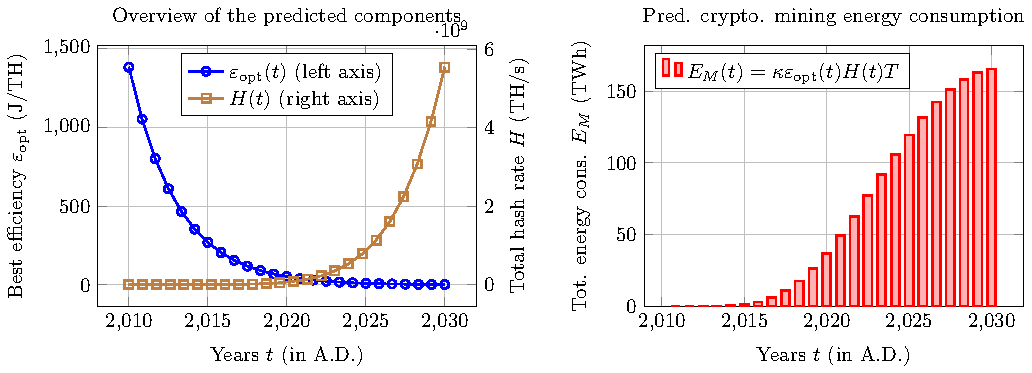
\includegraphics{figures/trends/crypto_energy.pdf}
\end{figure}

\subsubsection{The effects of change in energy mix}

Previously, we calculated the energy mix of each country $\boldsymbol{\zeta}$ from the dataset offered by IEA. These values also vary over time. We plot an extract of the trends of some countries and sub-regions in Figure \ref{fig_mix_data}. The changes in proportions of the three energy sources all follow a linear relationship.

With the observation on the data, we utilize linear regression to model the trend of each energy source's proportion of each country from the data of year 2010 to 2022.

\begin{figure}[!t]
	\centering
	\caption{Some example countries' and sub-regions' energy mix trend from year 2010 to 2022.}
	\label{fig_mix_data}
	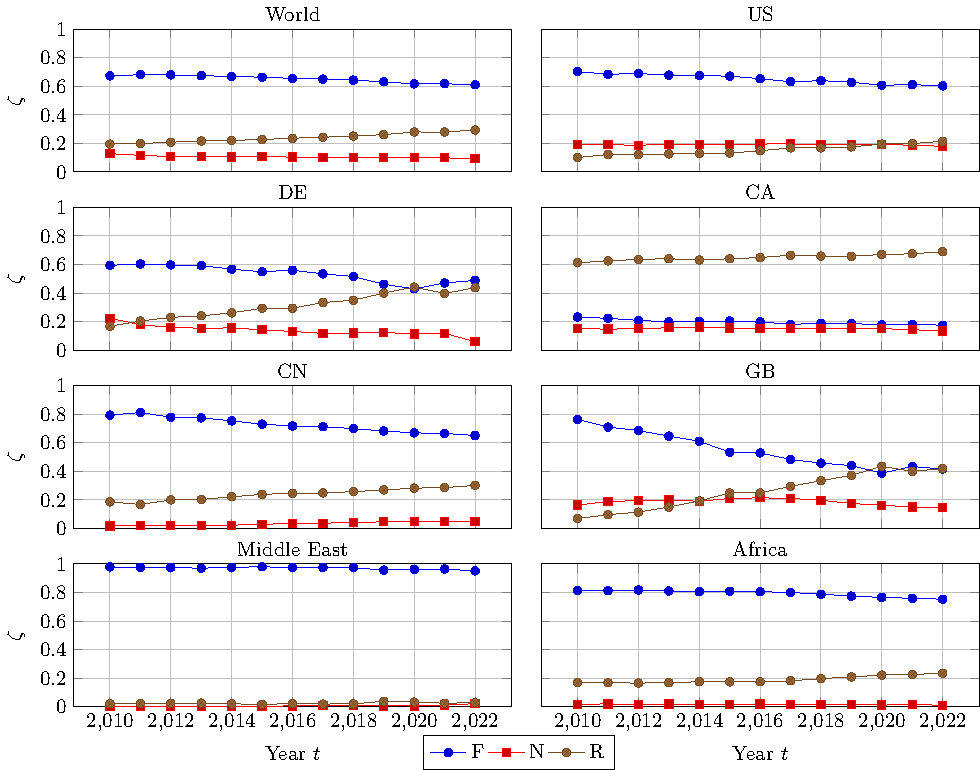
\includegraphics{figures/mix/mix.pdf}
\end{figure}

\bibliographystyle{apalike}
\bibliography{bib.bib}

\end{document}